\subsection{Sprint 6: Gestión de Postulaciones}
    \begin{description}
        \item \textbf{Duración}: 15 días.
        \item \textbf{Inicio del sprint }: 11 de marzo de 2022.
        \item \textbf{Cierre del sprint }: 25 de marzo de 2022.
    \end{description}

    \subsection{Planeación}

Esta iteración tuvo como propósito implementar un mecanismo para gestionar las postulaciones de los usuarios registrdos dentro del 
sistema, las actividades realizadas fueron:
\begin{enumerate}
    \item Se diseñó e implementó las interfaces de usuario para la gestión de posutlaciones según el tipo de cuenta.
    \item Se especificaron los requerimientos mediante casos de uso con sus respectivas interfaces de usuario.
    \item Se elaboró el diagrama de casos de uso para este sprint.
    \item Se elaboró la maquina de estados de una postulaciones.
\end{enumerate} 

Los requerimientos funcionales de este sprint se muestran en la siguiente tabla.
\begin{requerimientos}{funcionales}
    \RFitem{RF-14}{Postularse a vacantes}{El sistema debe permitir a los usuarios registrados enviar postularse a  las vacantes que esté abiertas.}
    \RFitem{RF-15}{Consultar el estado de postulaciones}{El sistema debe permitir al actor consultar el estado de su o sus postulaciones que haya hecho.}
    \RFitem{RF-16}{Dar seguimiento a postulaciones}{El sistema debe permitir al actor indicar  el estado de las postulaciones que tiene según sus vacantes publicadas.}
    \RFitem{RF-17}{Consultar postulaciones}{El sistema debe permitir a los actores registrados consultar las postulaciones que se hayan hecho de acuerdo a cada vacante.}
        
\end{requerimientos}
Los casos de uso que se describieron en este sprint pertenecen al \textbf{Módulo Postulaciones (PST)} cuyo propósito es gestionar
todas las postulaciones realizadas de candidatos para los reclutadores.

En la figura \ref{dcu:DCUPST} se puede ver el diagrama de casos de uso.
\begin{itemize}
    \item Los casos de uso \IUazul{} , son aquellos que se van implementar en este sprint.
    \item Los casos de uso \IUblanco{}, se tienen planeados para sprints posteriores.
\end{itemize} 

\begin{figure}[H]
    \begin{center}
        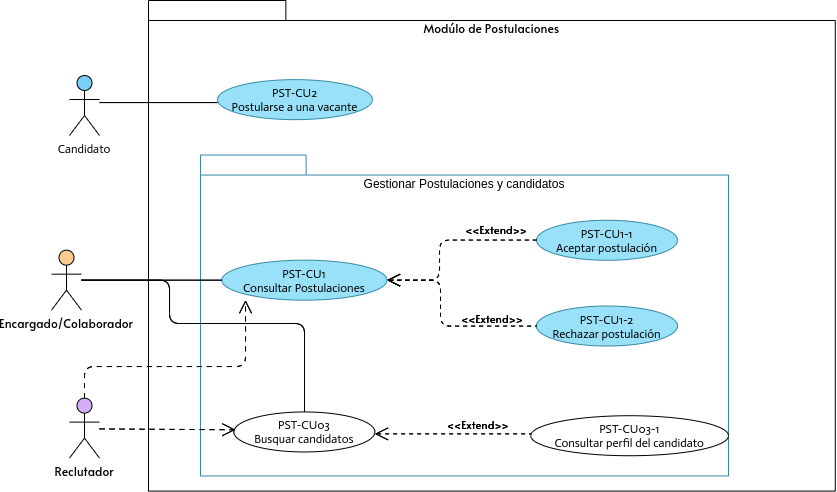
\includegraphics[width=.7\textwidth]{sprints/imagenes/DCUPST.png}
    \end{center}
    \caption{Diagrama de casos de uso del \textit{Modúlo Postulaciones}.}
    \label{dcu:DCUPST}
\end{figure}

Los casos de uso que se implementaron en este sprint fueron:
\begin{enumerate}
    \item PST-CU1 Consultar postulaciones
    \item PST-CU2 Postularse a una vacante
    \item PST-CU1-2 Rechazar postulación
\end{enumerate} 


\subsection{Ejecución}

Para la construcción del módulo de gestión de postulaciones se construyeron servicios para realizar la comunicación entre frontend y backend, y de esta forma hacer la petición HTTP con el verbo GET a cada endpoint que almacena la información de una postulación, ya sea las de postulaciones que realiza un candidato a una vacante o la lista postulaciones de candidatos que recibe el reclutador.
